\chapter{Marco Metodológico}

\section{Tareas comprendidas y no comprendidas}
Tareas comprendidas:

\begin{itemize}

\item Componente principal con servicios web, endpoints exponiendo scripts de control y
configuración de interruptores inteligentes, además de la inclusión del asistente personal.

\item Creación de red con permisos de autenticación, permitiendo la interacción segura entre los componentes.

\item Aplicaciones web y móvil para control y configuración de los periféricos.

\item Firmware optimizado a bajo nivel para permitir su ejecución en los sistemas de recursos limitados.

\item Investigación de tecnologías de comunicación, lenguajes de programación,
microcomputadoras y controladores orientados a IoT.

\item La presentación del dispositivo será en el protector normal del raspberry.

\end{itemize}

Tareas no comprendidas:

\begin{itemize}

\item Configuración inalámbrica de interruptores inteligentes.

\item Proceso de flasheo en masa de módulos de comunicación.

\item Compatibilidad de aplicación móvil con más de un SO.

\item Plan de importación de hardware para producción.

\item Investigación de patentes.

\end{itemize}

\section{Entregables}
\begin{table}[H]
\begin{tabular}{p{0.2\textwidth}p{0.3\textwidth}p{0.3\textwidth}p{0.2\textwidth}}
\toprule 
\textit{Título} & \textit{Descripción} & \textit{Tareas comprendidas} & \textit{Fecha de entrega} \\
\midrule \\
\rowcolor{green!5} Entrega de Cálculos / Rutinas con justificación de avance de 50 \% & Conectividad de interruptores y central de control. & Se investigaron las opciones para implementar la comunicación y control de los dispositivos sin una interfaz amigable y desarrollo del servidor web para conexión con Sonoff. Pruebas con Sonoff. & 15/11/2017 \\
Entrega Borrador del Informe del PFC & Realización de documento donde se registran las investigaciones, decisiones y desarrollos.
 & Se realizó la conexión con la aplicación móvil, así como una implementación mínima del asistente personal. & 14/12/2017 \\
\rowcolor{green!5} Entrega de Cálculos \/ Rutinas con justificación de avance de 100 \% & Prototipo del sistema finalizado & Conexión de los periféricos con el servidor central, órdenes de servidor para apagar y prender los periféricos, integración del servidor con el asistente personal, descubrimiento de todos los dispositivos de la red, scipts de voz generales. & 14/02/2018 \\
\bottomrule
\end{tabular}
 \caption{\textit{Entregables: descripción y fecha}}
\end{table}

\section{Restricciones: Tiempo, presupuesto, tecnología}

Entre las restricciones más relevantes para el alcance del proyecto se encuentran la necesidad de obtener como resultado un interruptor inteligente de tamaño reducido, capaz de ser colocado en el espacio destinado a las llaves de corriente convencionales y coste competitivo con los productos en el mercado actual. 

Sumado a esto, se tiene que los módulos de comunicación que cumplen las características anteriores utilizan protocolos en desarrollo, algunos de los cuales funcionan con frecuencias similares a las reservadas para otros servicios, por lo que se deberá estudiar cuál de estos es posible utilizar en Uruguay.

Otra consideración a tener en cuenta es el rango máximo de comunicación entre dispositivos, siendo que dependiendo del protocolo y módulo elegido se deberá balancear entre velocidad de transmisión, penetración en estructuras físicas (paredes, muebles, rejas) y consumo de energía.

Se deberá utilizar hardware y software con licencias de libre modificación y distribución, ya que el uso de productos pagos repercutiría de manera negativa en la accesibilidad del producto al público en general, provocando que el impacto en la sociedad.

Al contar con un límite de 4 pedidos de un máximo de USD 200, esta realidad conlleva a que, en caso de no ser capaces de incluir algún módulo o componente, nos veremos obligados a descartar dicha alternativa.

\section{Supuestos y riesgos}

El itinerario y alcance del proyecto se planean con el supuesto de la puntualidad de los pedidos al exterior; ya que, tratándose de state-of-the-art hardware, el mismo no está disponible en Uruguay, o en caso de estarlo, su precio es varias veces mayor al cual se comercializa en el exterior. 

Dentro de los posibles interesados en el proyecto se encuentra UTE. Al ser un ente público se consideró que puede demorar en brindar la información que se solicita para adaptar el modelo a este interesado. Si este fuere el caso, se desistirá de este ente para realizar en el modelado del producto.

También es posible que alguno de los componentes se rompa por un mal uso dada la poca experiencia con este tipo de dispositivos o que el mismo venga fallado. Si esto sucediese se deben comprar dispositivos nuevos lo cual conllevará contratiempos por el envío de los materiales. Para aliviar riesgo, dado que los elementos de este proyecto no son caros y pueden ser reusados, se compraran de forma  redundante para que el fallo en alguno de los elementos no golpee al proyecto.

\section{Estructura de Desglose de Trabajo (EDT)}

\begin{figure}[h]
  \centering
  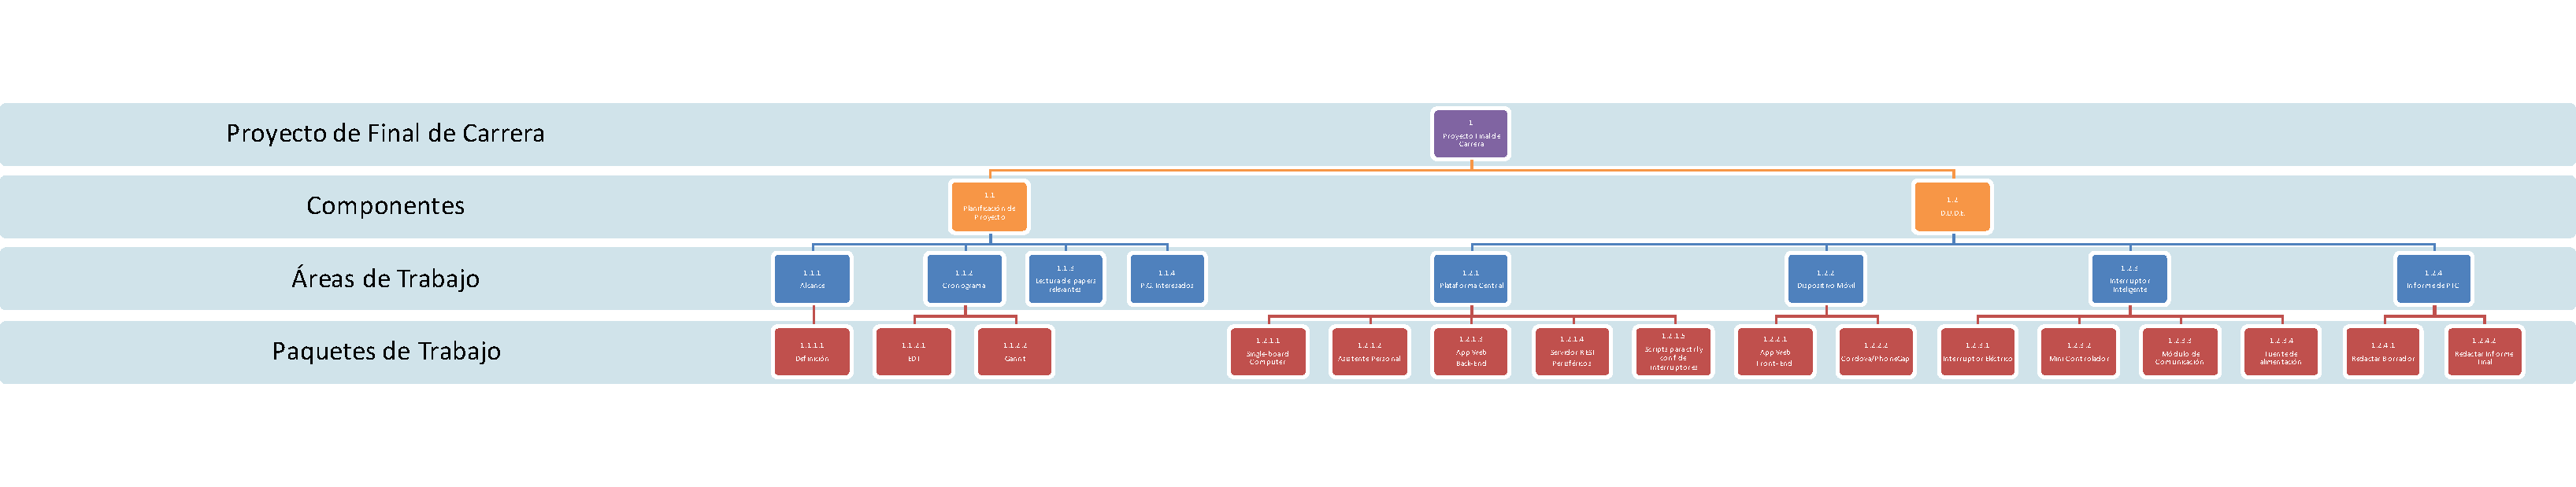
\includegraphics[width=\textwidth, keepaspectratio]{images/EDT}
  \caption{\textit{Estructura de Desglose de Trabajo.}}
  \label{fig:edt}
\end{figure}

\section{Desglose de Paquetes de Trabajo en Actividades}

\section{Procedimientos}

\subsection{Protocolos}
La elección de protocolos consistió en dos rondas, donde el primer acercamiento fue absolutamente teórico, se basó en la investigación por medio de papers y de la documentación oficial en Internet de los protocolos, para descartar varios de ellos, y así reducir el número de posibilidades.
Luego se investigó implementaciones y hardware disponible para los protocolos elegidos, siendo esta una investigación más práctica, donde se tuvo en cuenta la calidad y madurez de las librerías desarrolladas para cada uno, así como el acceso y precio de los módulos correspondientes. Otro punto importante al momento de decidir fue la comunidad creada alrededor de los protocolos y plataformas de desarrollo, ya que se sabía que su apoyo sería indispensable para reducir la curva de aprendizaje y evitar caer en errores comunes sin tener una fuente rápida y efectiva para despejar dudas.

\subsection{Librerías}

Respecto a las librerías, se buscó trabajar librerías maduras y mantenidas, que no estén abandonadas por sus mantenedores y cuyos issues hayan o estén siendo resueltos.
La razón de por qué utilizar librerías y no desarrollar las funcionalidades por nosotros mismos son simples, en el caso de encontrar una librería que se adecúe a las necesidades del proyecto y con las características buscadas mencionadas, no tiene caso reinventar la rueda. Esto es teniendo en cuenta la revisión de las mismas y que hay un entendimiento de cómo funcionan, y no es simplemente una caja negra. Es una de las intenciones la mejora de las mismas, ya que se interactuó con sus mantenedores, abriendo issues y ayudando a la mejora de estas.
El procedimiento para la investigación y adaptación de las librerías en el sistema sigue los siguientes lineamientos:

\begin{itemize}

\item Análisis del estado de la librería:

	\begin{itemize}

	\item Cantidad de commits.
	\item Issues abiertos y resueltos.
	\item Últimas actualizaciones.
	\item Cantidad de versiones.
	\item Comentarios y stars que tenga el repositorio.
	\item Calidad de documentación.
	\item Cantidad y calidad de ejemplos.
	\item Menciones y utilización de la librería en proyectos.
	\item Requerimientos de hardware.

	\end{itemize}

\item Revisión de código y ejemplos:

	\begin{itemize}

		\item Entendimiento general de las funciones brindadas por la librería.
		\item Lectura de ejemplos relevantes para el proyecto, usualmente comenzando con el "Hello World", para entender el uso básico de la librería y luego proseguir con uno que utilice las funcionalidades que se utilizarán en el proyecto.

	\end{itemize}

\item Instalación de la librería y experimentación con ejemplos:

	\begin{itemize}

	\item Instalación de librería en un ambiente virtual para evitar conflictos de librerías utilizadas por la que se está investigando y las que utilizan distintas partes del sistema.
	\item Utilizar el ejemplo básico para comprobar que la instalación fue correcta.
	\item Experimentar con el ejemplo que utilice las funciones en las que se está interesado.
	\item Implementar una solución para el sistema con la librería.
	\item Acoplar dicha solución al sistema.

	\end{itemize}

\end{itemize}

\subsection{Hardware}

Los procedimientos de desarrollo con hardware fueron los menos consistentes debido a las grandes diferencias de los mismos, por lo que se detallan por separado.

\subsubsection{Raspberry Pi}

El componente era previamente conocido y es el más fácil de manejar en este contexto, ya que es posible utilizar git para clonar y actualizar el código existente en el componente. Además de esto es posible modificar los archivos desde una sesión ssh, permitiendo probar cambios en el dispositivo antes de realizar commits. El procedimiento que se siguió para desarrollar código en este dispositivo es:

\begin{itemize}
\item Desarrollo y testeo de código en el computador personal.
\item Si se está desarrollando un nuevo módulo: subir el código a GitHub y hacer un pull desde el Raspberry Pi.
\item En caso de realizar modificaciones pequeñas, se copia el código por ssh al archivo del Raspberry Pi y se testea antes de versionar los cambios.
\item Una vez terminado el testeo, proceder a realizar un Pull Request y volver a hacer un pull de la branch dev en el Raspberry Pi.

\end{itemize}

\subsubsection{Sonoff}

Los pasos para su preparación fueron los siguientes:

\begin{itemize}

\item Compra y espera de entrega. Se realizaron dos compras, una express de 2 unidades y otra de envío gratuito con 9 unidades, una de ellas un Sonoff Dual.

\item Adaptación física para desarrollo, se soldaron las conexiones y se confeccionó un switch físico para poder reiniciar fácilmente el dispositivo.

\item Una vez conectado por el adaptador USB/Serial, se borran los SPIFFS con la herramienta esptool.

\item Se resetea el Sonoff con el botón presionado para entrar en modo configuración.

\item Con Atom y el plug-in de PlatformIO se flashea el firmware desarrollado al componente.

\end{itemize}





